\section{Particle Cross Sections}
\subsection{Review of results + Mandelstam variables}
To summarize what we have derived thus far:
\begin{itemize}
    \item One can isolate the non-trivial part of the S-matrix as:
    \begin{equation}
        \braket{f}{i} = \delta_{if} + iT_{if}
    \end{equation}
    or $S = 1 + iT$.
    \item Translation invariance further implies that:
    \begin{equation}
        iT_{if} = (2\pi)^4\delta^4(k_1 + k_2 - k_1' - k_2')i\mathcal{M}(k_1, k_2 \to k_1', k_2')
    \end{equation}
    \item We studied $\mathcal{M}$ for two interacting theories, at tree-level:
    \begin{itemize}
        \item $\mathcal{L}_{\text{int}} = -\frac{\lambda}{4!}\phi^4$, with the diagram:
        \begin{center}
            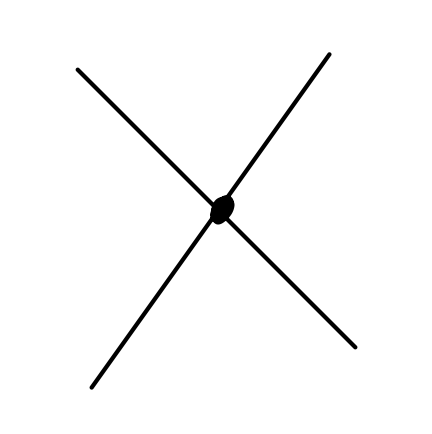
\includegraphics[scale=0.4]{Lectures/Figures/lec18-Olambda.png}
        \end{center}
        and matrix element (independent of the momenta):
        \begin{equation}
            \mathcal{M}(k_1, k_2 \to k_1', k_2') = -\lambda
        \end{equation}
        \item $\mathcal{L}_{\text{int}} = -\frac{g}{3!}\phi^3$, with diagrams:
        \begin{center}
            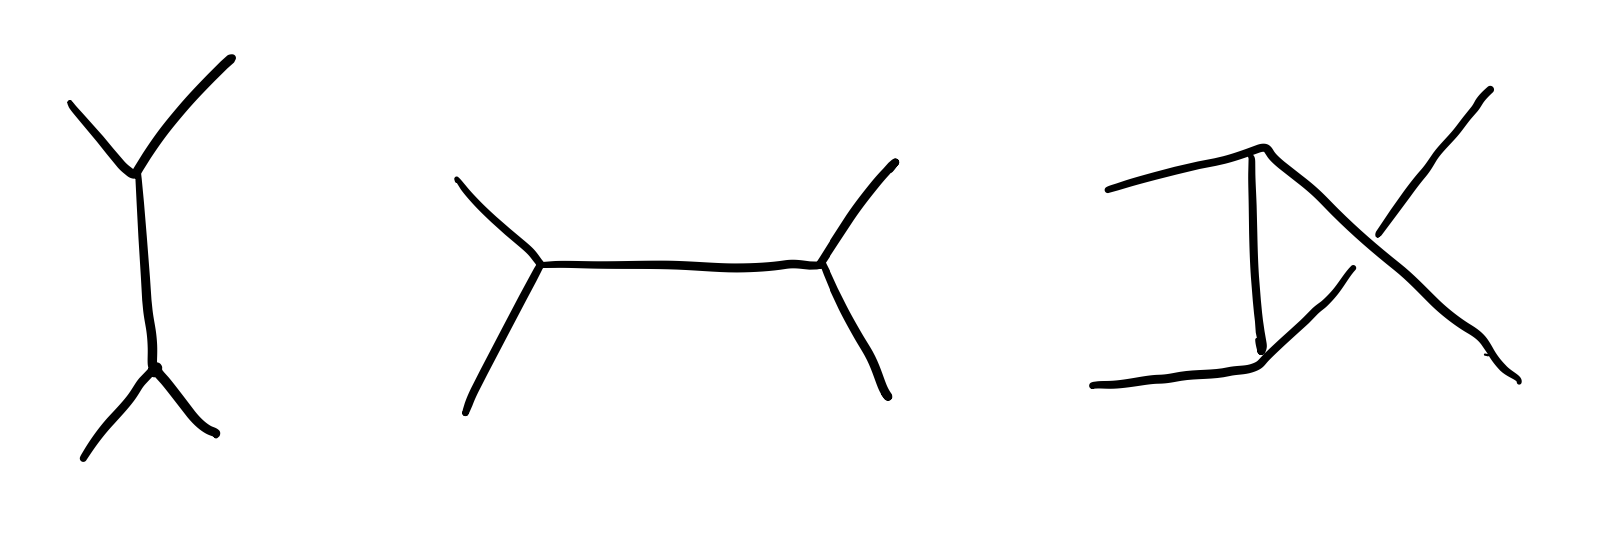
\includegraphics[scale=0.4]{Lectures/Figures/lec18-Ogsquared.png}
        \end{center}
        and matrix element (dependent on the momenta):
        \begin{equation}
            \begin{split}
                \mathcal{M}(k_1. k_2 \to k_1', k_2') &= g^2\left[\frac{1}{(k_1 + k_2)^2 + m^2} + \frac{1}{(k_1 - k_1')^2 + m^2} + \frac{1}{(k_1 - k_2')^2 + m^2}\right] 
                \\ &= g^2\left[\frac{1}{m^2 - s} + \frac{1}{m^2 - t} + \frac{1}{m^2 - u}\right]
            \end{split}
        \end{equation}
        where $s, t, u$ are the \emph{Mandelstam variables}:
        \begin{equation}
            s = -(k_1 + k_2)^2, t = -(k_1 - k_1')^2, u = -(k_1 - k_2')^2
        \end{equation}
        and are the only Lorentz invariant variables that the S-matrix can depend on. Why are these the only three? First, note that the fourth momenta is fixed by the $\delta$ function, so it can depend on at most three particles. Then, further noting that $k_1^2 = k_2^2 = k_1'^2 = k_2'^2 = -m^2$, (the S-matrix is on-shell) the only way to get nontrivial variables is by taking combinations. Further, there is actually a relation between the three, so it is really only 2 that are independent:
        \begin{equation}
            s + t + u = 6m^2 - 2k_1(k_2 - k_1' - k_2') = 6m^2 - 2k_1(-k_1) = 6m^2 + 2k_1^2 = 4m^2
        \end{equation}
        where in the second equality we use the delta function. Since their sum is fixed, there are only 2 independent variables, e.g. $s, t$. But sometimes it is convenient to keep the third ($u$) around (instead of writing it as $u = 4m^2 - s - t$) as it keeps the crossing symmetry (that is, symmetry under swaps of $s/t/u$) manifest in our results.
    \end{itemize}
\end{itemize}

As an aside; here we compute the S-matrix perturbatively, but there is a research program known as the ``S-matrix bootstrap'' which is a non-perturbative approach to QFT, which essentially guesses possible matrix elements $\mathcal{M}(s, t, u)$ using all of the properties that they have to satisfy - crossing symmetry, analyticity, causality, Lorentz invariance. This program was born out of study of strongly coupled QFTs (e.g. QCD) and was abandoned for a while, but is now seeing a resurgence.

\subsection{Converting matrix elements to cross sections}
This is the last topic we will cover in this course! It is discussed in Section 10 of Srednicki, 5.1 of Schwartz, and 4.6 of Peskin. The former 2 have a slightly heuristic/faster derivation, Peskin has a slightly more careful derivation.

The cross sectional area of an object is the area $\sigma$ that we can see of an object, e.g. the 2-D ball below has a classical cross sectional area of $\sigma = 2\pi r$. 

\begin{center}
    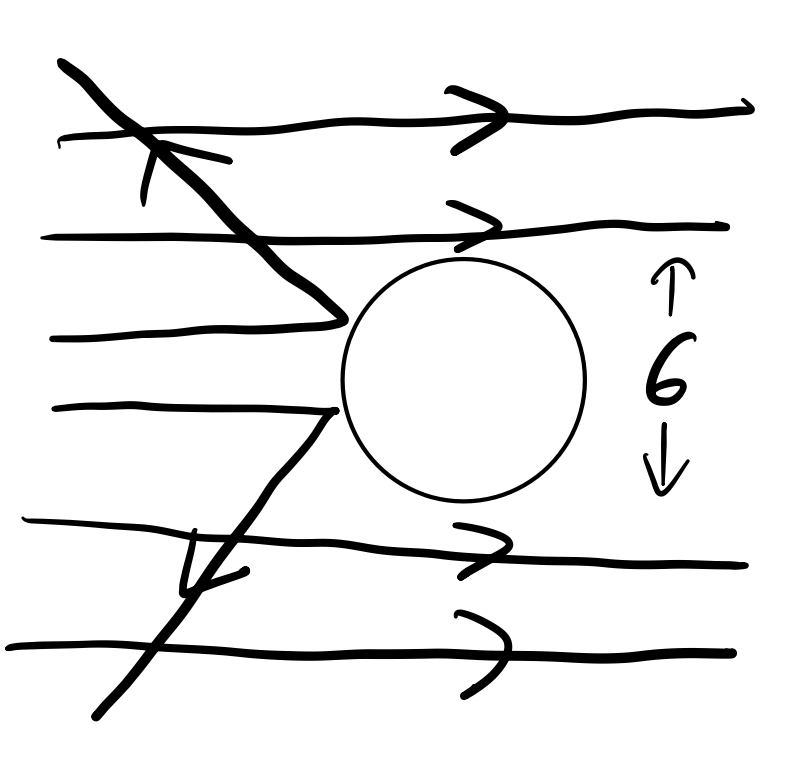
\includegraphics[scale=0.35]{Lectures/Figures/lec18-sigma.png}
\end{center}

We can probe what $\sigma$ is by scattering objects off of it. Consider shooting a bunch of particles at an object, then the number of scattered particles in some time $T$ is given by:
\begin{equation}
    N_{\text{scatter}} = \sigma v T n
\end{equation}
where $\sigma$ is the cross section, $v$ is the speed of the particles, and $n$ is the number density. Thus:
\begin{equation}
    \sigma = \frac{N_{\text{scatter}}}{vTn}
\end{equation}
this is the classical definition of a cross section - in QM, we instead define it as the probability to scatter. Thus, in QFT the cross section is not only a measure of the size of a particle, but also how strongly it interacts.

In addition to just the cross section/total probability, we would also like to resolve the possible outgoing states. Thus, we look at the differential cross section:
\begin{equation}
    d\sigma = \frac{dP}{vT n}
\end{equation}
with $dP$ the differential probability to scatter into a state with a given $k_1', k_2'$. This formula has to be taken with a slight grain of salt, because in the thermodynamic limit ($V \to \infty$) $dP$ and $n$ both go to zero (the former because the probability for scattering into a specific momenta is zero, the latter because $n = \frac{N}{V} \to 0$). Thus, it is useful to temporarily introduce $V < \infty$, and take the density to be $n = \frac{1}{V}$ (looking at scattering off of a single-particle).

We study the differential probability:
\begin{equation}
    dP = \frac{\abs{\braket{f}{i}}^2}{\braket{i}{i}\braket{f}{f}}d\Pi; \quad d\Pi = \prod_{i=1}^n \frac{V^3 d^3k_i'}{(2\pi)^3}
\end{equation}
where $d\Pi$ accounts for a generalization to $2 \to n$ scattering. We can calibrate the normalization of this expression using the free theory (working in $D = 3 + 1$ dimensions, and for $2\to2$ scattering for simplicity):
\begin{equation}
    \braket{f}{i} = 2\e_{k_1}2\e_{k_2}(2\pi)^6\delta^3(k_1 - k_1')\delta^3(k_2 - k_2')
\end{equation}
\begin{equation}
    \braket{i}{i} = 2\e_{k_1}2\e_{k_2}(2\pi)^3\delta^3(0)\delta^3(0)
\end{equation}
\begin{equation}
    \braket{f}{f} = 2\e_{k_1'}2\e_{k_2'}(2\pi)^3\delta^3(0)\delta^3(0)
\end{equation}
Then:
\begin{equation}
    \int dP = \frac{(\delta^3(\v{k}_1 - \v{k}_1')\delta^3(\v{k}_2 - \v{k}_2'))^2}{(\delta^3(0)\delta^3(0))^2}\int d\Pi = \int\frac{(\delta^3(\v{k}_1 - \v{k}_1')\delta^3(\v{k}_2 - \v{k}_2'))^2}{(\delta^3(0)\delta^3(0))^2}\left(\frac{V}{(2\pi)^3}\right)^2 d^3k_1' d^3k_2' = \left(\frac{V}{(2\pi)^3\delta^3(0)}\right)^2 = 1
\end{equation}
So the normalization is indeed correct.

More generally for $2 \to n$:
\begin{equation}
    \braket{f}{f} = \prod_{i=1}^n 2\e_{k_i'}(2\pi)^3\delta^3(0) =  \prod_{i=1}^n 2\e_{k_i'}V
\end{equation}
\begin{equation}
    \braket{i}{i} = 2\e_{k_1}2\e_{k_2}(2\pi)^3\delta^3(0)\delta^3(0)
\end{equation}
Then looking at the overlap:
\begin{equation}
    \abs{\braket{f}{i}}^2 = (2\pi)^4\delta^4(0)(2\pi)^4\delta^3(k_1 + k_2 - \sum_{i=1}^n k_i')\abs{\mathcal{M}}^2
\end{equation}
where $(2\pi)^4\delta^4(0) = VT$. Thus looking at the differential probability:
\begin{equation}
    dP = \frac{VT(2\pi)^4\delta^4(k_1 + k_2 - \sum_{i}k_i')\abs{\mathcal{M}}^2}{2\e_{k_1}2\e_{k_2}V^2\prod_{i=1}^n(2\e_{k_i'}V)}\prod_{i=1}^n\frac{Vd^3k_i'}{(2\pi)^3} = \frac{T\abs{M}^2}{V(2\e_{k_1})(2\e_{k_2})}\left((2\pi)^4\delta^4(k_1 + k_2 - \sum_i k_i')\prod_i \frac{d^3k_i'}{(2\pi)^32\e_{k_i'}}\right)
\end{equation}
where the expression in brackets is the Lorentz-invariant phase space measure:
\begin{equation}
    d\Pi_{\text{LIPS}} = (2\pi)^4\delta^4(k_1 + k_2 - \sum_i k_i')\prod_i \frac{d^3k_i'}{(2\pi)^32\e_{k_i'}}
\end{equation}
Cross-sections are generally not Lorentz invariant, but it is nice to factor out this part that is.

Thus, returning to the differential cross section:
\begin{equation}
    d\sigma = \frac{\abs{\mathcal{M}}^2}{(2\e_{k_1})(2\e_{k_2})\abs{\v{v}_1 - \v{v}_2}}d\Pi_{\text{LIPS}}
\end{equation}
where the velocity is the group velocity:
\begin{equation}
    \v{v}_i = \dod{\e_{k_i}}{\v{k}_i} = \dod{\sqrt{\v{k}_i^2 + m^2}}{\v{k}_i} = \frac{\v{k}_i}{\e_{k_i}}
\end{equation}

We saw that $\abs{\mathcal{M}}$ was proportional to (some power of) the coupling, so as we stated previously, the cross-section is indeed a measure of the interaction.

\subsection{Evaluating 2-2 Differential Cross Section}
Lets consider a $\phi\phi \to \phi\phi$ scattering. 

\begin{center}
    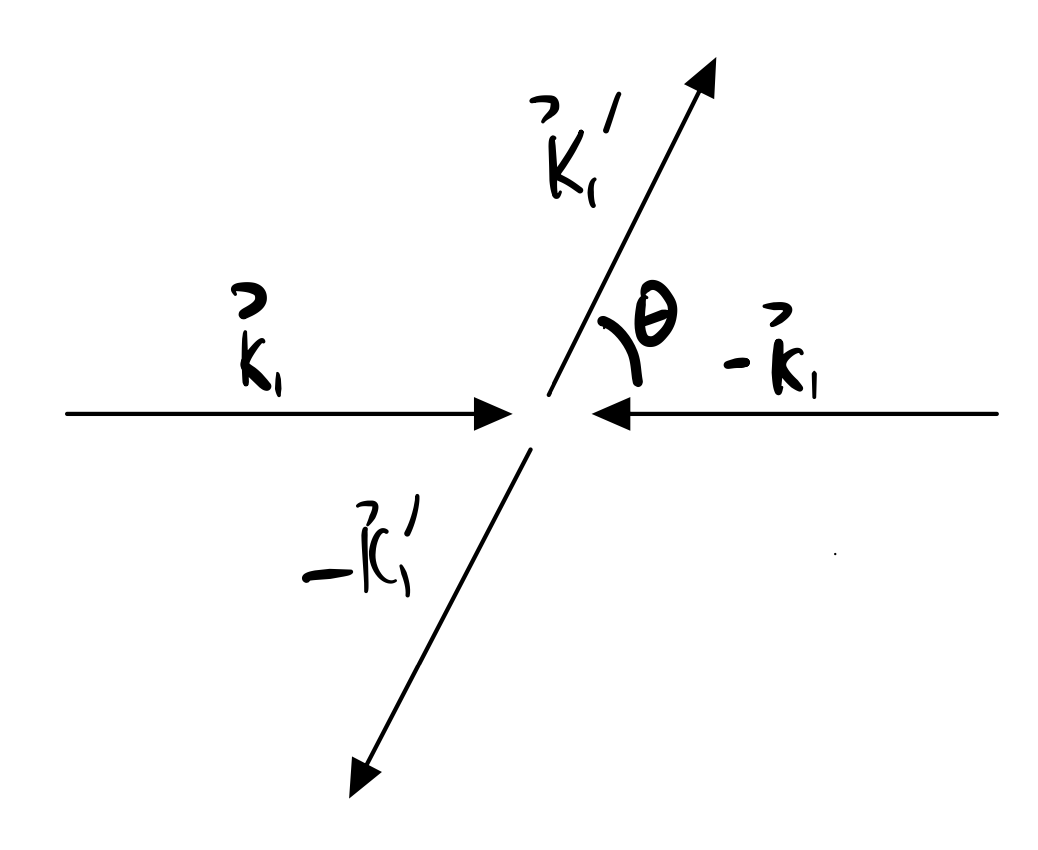
\includegraphics[scale=0.35]{Lectures/Figures/lec18-scatter.png}
\end{center}

In the CoM frame, $\v{k}_1 = -\v{k}_2$ (and thus $\e_{\v{k}_1} = \e_{\v{k}_2}$). The total centre-of-mass frame energy is $E_{CM} = 2\e_{\v{k}_1}$. By momentum conservation, $\v{k}_2' = -\v{k}_1'$, and by energy conservation $2\e_{k_1} = 2\e_{k_1'}$ and so:
\begin{equation}
    \abs{\v{k}_1} = \abs{\v{k}_2} = \abs{\v{k}_1'} = \abs{\v{k}_2'}
\end{equation}
Thus the only free parameters in this problem is the norm of the momentum vector $\abs{\v{k}_1}$ and the angle of scattering $\theta$. These map to the Mandelstam variables $s$ and $t$. 

We need to put together the Lorentz-invariant phase space measure. We will see that we shall be able to remove some of the differentials.
\begin{equation}
    d\Pi_{\text{LIPS}} = (2\pi)^4\delta^4(k_1 + k_2 - k_1' - k_2')\frac{d^3k_1'}{(2\pi)^32\e_{k_1'}}\frac{d^3k_2'}{(2\pi)^32\e_{k_2'}}
\end{equation}
We can start by integrating out $\v{k}_2'$, which converts the 4-momentum conservation from the dirac delta to an energy conservation dirac delta:
\begin{equation}
    d\Pi_{\text{LIPS}} = (2\pi)\delta^4(\e_{k_1} + \e_{k_2} - \e_{k_1'} - \e_{k_2'})\frac{d^3k_1'}{(2\pi)^3(2\e_{k_1'})(2\e_{k_2'})}
\end{equation}
in the COM frame (this is a LI quantity, so we can evaluate it in any frame we like) - we go into spherical coordinates, and the the $k_1'$s appearing below are now the magnitude of the momenta:
\begin{equation}
    d\Pi_{\text{LIPS}} = (2\pi)\frac{\delta(E_{CM} - 2\e_{k_1'})}{(2\pi)^3E^2_{CM}}k_1'^2 dk_1' d\Omega
\end{equation}
The $\delta$ function fixes $\e_{k_1'} = \frac{E_{CM}}{2}$ and so fixes $k_1' = k_1$. Thus using the usual trick of the Jacobian and delta functions:
\begin{equation}
    \delta(E_{CM} - 2\e_{k_1'}) = \delta(2k_1 - 2k_1')\frac{1}{\dod{\e_{k_1'}}{k_1'}} = \frac{1}{2}\delta(k_1 -k_1')\frac{1}{v_i}
\end{equation}
Thus:
\begin{equation}
    d\Pi_{\text{LIPS}} = \frac{1}{2}\frac{1}{v_1}\frac{1}{(2\pi)^2E_{CM}^2}k_1^2d\Omega
\end{equation}
and then recalling that $v_1 = \frac{k_1}{\e_{k_1}}$, it follows that $k_1 = v_1\e_{k_1}$ and so $\e_{k_1} = v_1\frac{E_{CM}}{2}$:
\begin{equation}
    d\Pi_{\text{LIPS}} = \frac{v_1}{32\pi^2}d\Omega
\end{equation}
which is our result for the measure. It is dimensionless as it should be. It is not manifestly Lorentz invariant (an artifact of choosing a reference frame to evaluate), but contains both $v, d\Omega$ which together enforces its Lorentz invariance. Plugging this into our formula for the differential cross section:
\begin{equation}
    d\sigma = \frac{\abs{\mathcal{M}}^2}{(2\e_{k_1})(2\e_{k_2})\abs{\v{v}_1 - \v{v}_2}}d\Pi_{\text{LIPS}} = \frac{\abs{\mathcal{M}}^2}{64\pi^2E_{CM}^2}d\Omega
\end{equation}
Thus we obtain the differential cross section:
\begin{equation}
    \boxed{\dod{\sigma}{\Omega_{CM}} = \frac{\abs{\mathcal{M}}^2}{64\pi^2 E_{CM}^2}}
\end{equation}
which is also known as the ``angle-resolved differential cross section''.

As a note, the above expression is related to the Mandelstam variable $s$ as:
\begin{equation}
    s = -(k_1 + k_2)^2 \stackrel{COM}{=} (k_1^0 + k_2^0)^2 = (2\e_{k_1})^2 = E_{CM}^2
\end{equation}
where we use that the spatial parts of the momenta are zero in the COM frame. The other independent Mandelstam variable $t$ will be related to $\theta$. 

If we wanted the full cross section $\sigma$, we have to carry out the full integral over the angles $\Omega$. But this is non-trivial and depends on the particular physics/theory, and we have to take into account the angular dependence of the matrix element. Though - note that since there is no $\phi$ (azimuthal)-dependence here, we could carry out the azimuthal integral in $d\Omega = d\phi d\cos\theta$ which gives a factor of $2\pi$. Next quarter, we encounter particles with spin, and there we will see an azimuthal dependence as a result.

\subsection{Examples of 2-2 cross sections}
\begin{itemize}
    \item For $\mathcal{L}_{\text{int}} = -\frac{\lambda}{4!}\phi^4$, we have that $\mathcal{M} = -\lambda$ and so:
    \begin{equation}
        \dod{\sigma}{\Omega_{CM}} = \frac{\lambda^2}{64\pi^2 s}
    \end{equation}
    Here the matrix element is not dependent on the angle and we can carry out the angular integral. This yields a factor of $\frac{4\pi}{2}$ (the 2 comes about because we overcount the angles; there is a symmetry of reversing the angle), and thus:
    \begin{equation}
        \sigma = \frac{\lambda^2}{32\pi s}
    \end{equation}
    \item For $\mathcal{L}_{\text{int}} = -\frac{g}{3!}\phi^3$, we have $\mathcal{M}(s, t) = \mathcal{M}(s, \theta)$ so there is a nontrivial dependence of the matrix element on the angle and so the angular integral is more complicated. You will have fun with this in PS9.
\end{itemize}

If we go to higher orders in $\lambda$, we get the diagrams:

\begin{center}
    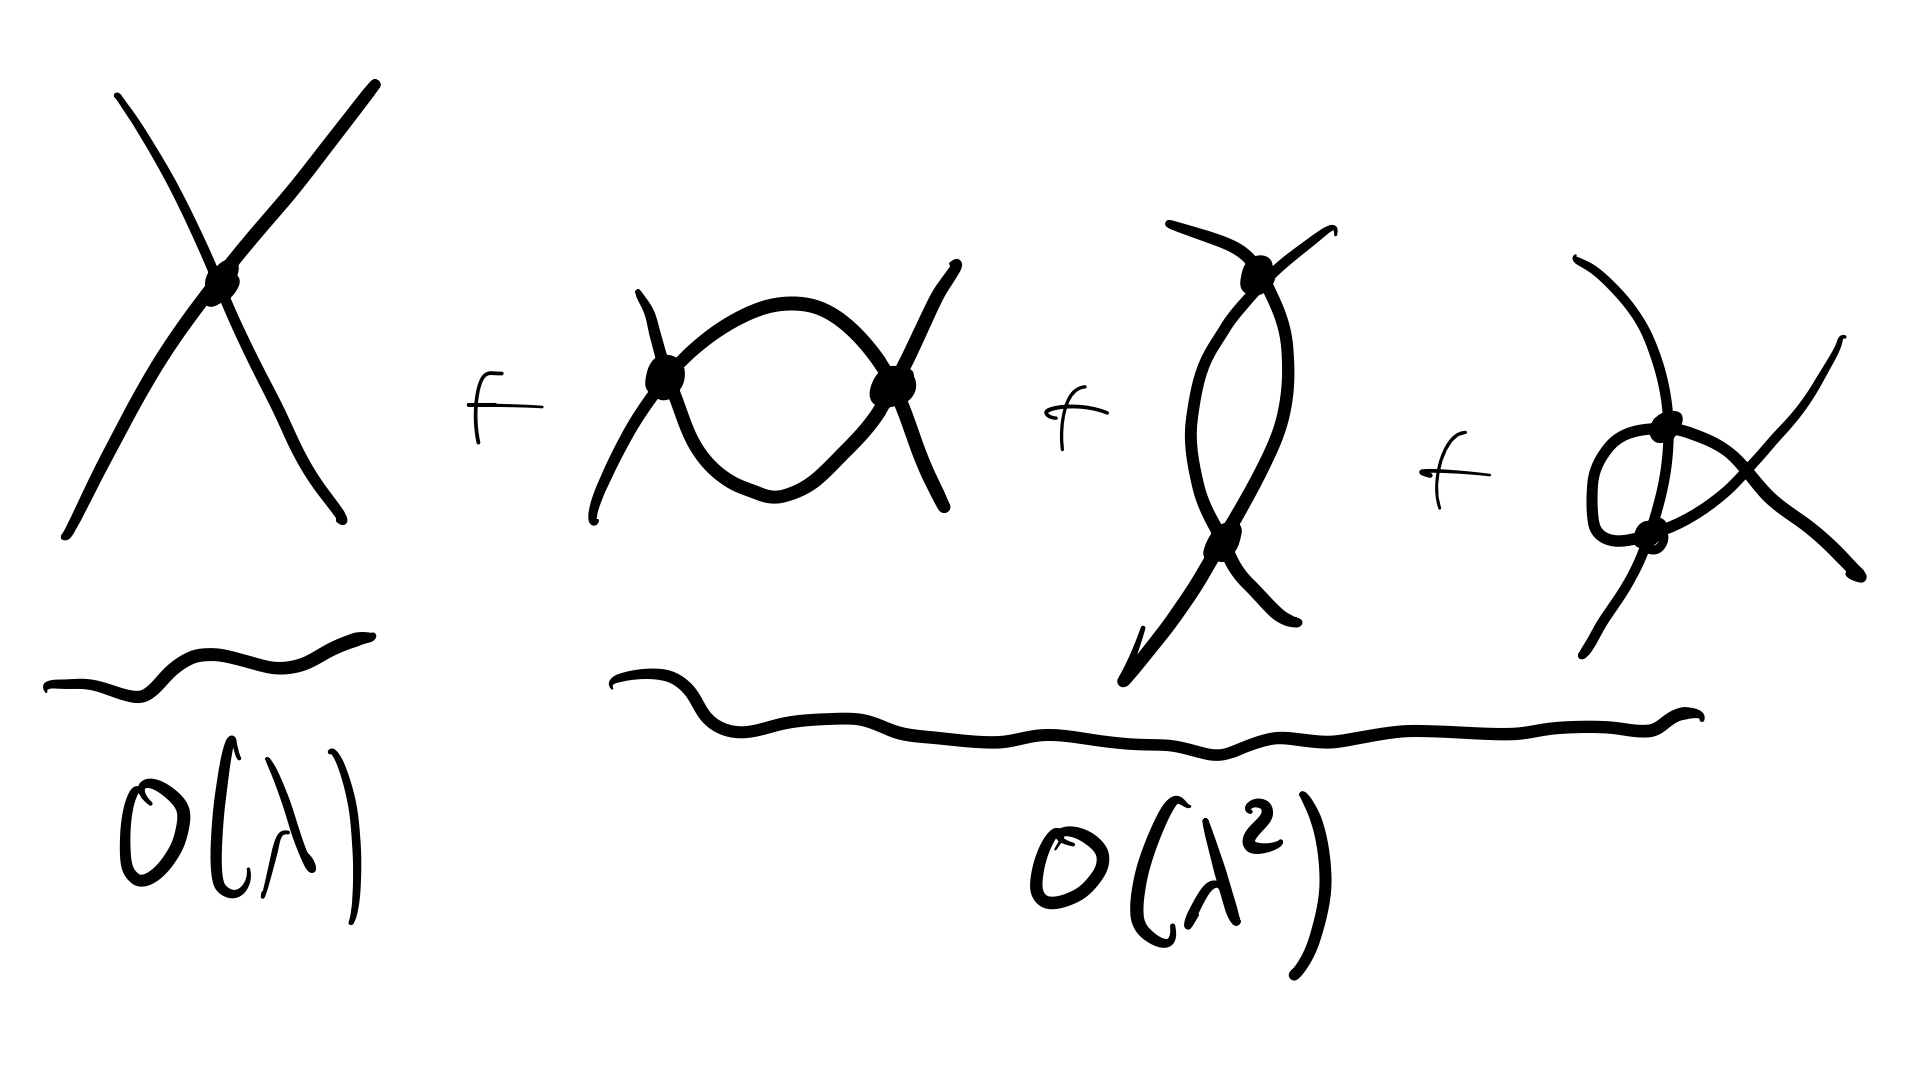
\includegraphics[scale=0.3]{Lectures/Figures/lec18-Olambdasquared.png}
\end{center}

which we know from our prior analysis gives the the matrix element picks up a logarithmic part:
\begin{equation}
    \mathcal{M} \sim \lambda(1 + \lambda \log s + \ldots)
\end{equation}
which via the RG procedure can be resummed:
\begin{equation}
    \mathcal{M} \stackrel{RG}{\to} \frac{\lambda}{1 - \lambda \log s}.
\end{equation}
this log correction to the cross section can be measured in experiment:

\begin{center}
    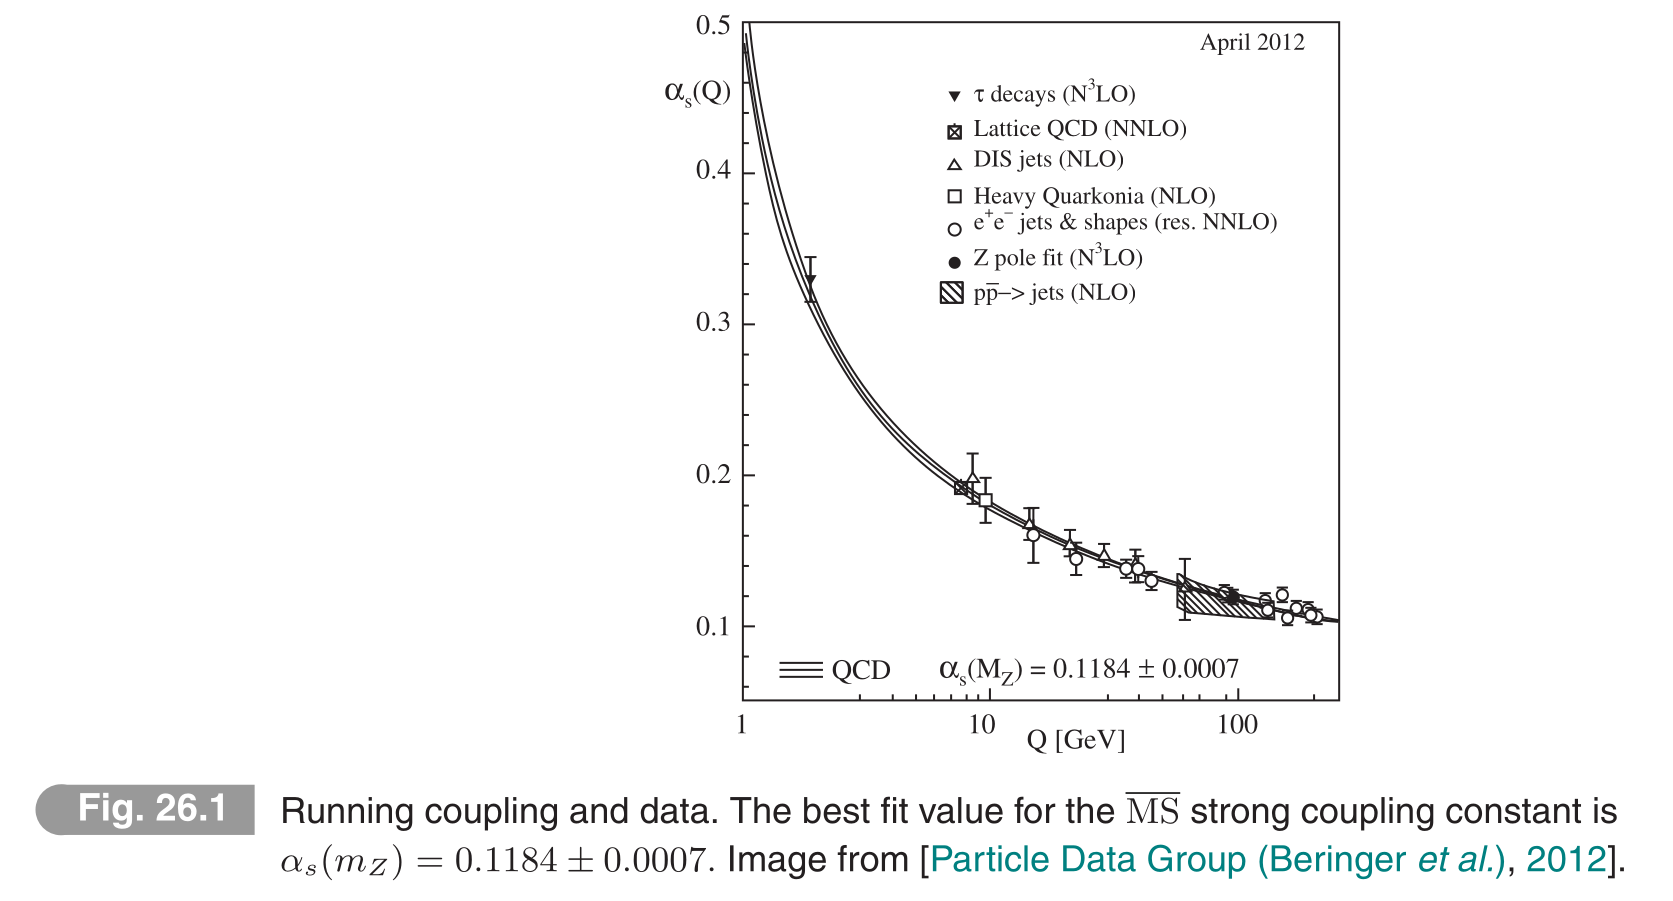
\includegraphics[scale=0.3]{Lectures/Figures/logruncouplings.png}
\end{center}

This brings us to the end of QFT1! This is not an easy topic, and one does not understand it after taking a single course. It is reccomended to take multiple classes/learn from multiple perspectives! It is also reccomended that you take QFT2. Here in QFT1 we explored scalar field theory very deeply, and learned a lot of deep results in QFT (e.g. non-perturbative results, renormalization group). In QFT2 we'll make up for the missing parts, like fermions, gauge fields, particles with spin.